%%% --------------------------------------------------------
%%> \section{Директиви компілятора}
%%% --------------------------------------------------------

% !TeX program = lualatex
% !TeX encoding = utf8
% !BIB TS-program = biber




\documentclass[]{iptconf}





%%% --------------------------------------------------------
%%> \section{Реєстраційна форма}
%%% --------------------------------------------------------
\regform{
    fullname = {Завалій Олександр Миколайович},          % Повне ім'я доповідача (перший автор)
    birthday = {13.03.2004},                    % Дата народження доповідача
    position = {студент},                      % Посада доповідача
    phone = {},                    % Телефонний номер доповідача
    authoremail = {olezav-ipt25@lll.kpi.ua},          % Email доповідача
    confsection = {Математичне моделювання та аналіз даних}, % Секція конференції,
    copynum = {0},                              % Замовлена число друкованого збірника
    needliving = {ні},                          % Потреба в житлі (Ні/Хостел/Готель/інше)
    needinvitanion = {ні},                      % Чи потрібне запрошення на конференцію?
}





%%% --------------------------------------------------------
%%> \section{Використані пакети}
%%% --------------------------------------------------------
\usepackage[most]{tcolorbox}
\usepackage{tabularray}
\UseTblrLibrary{booktabs}
\usepackage{amsmath}
\usepackage{dsfont}
\usepackage{mathrsfs}
\usepackage{wrapfig}
\usepackage{xurl}
\usepackage{tikz}
\usepackage{pgfplots}
\pgfplotsset{compat=1.18}
\usepackage{listings}





%%% --------------------------------------------------------
%%> \section{Файл бібліографії}
%%% --------------------------------------------------------
%% Змініть ім'я файлу бібліографі на ваш.
%% Краще, щоб його назва була така ж сама,
%% як у вашого .tex-файлу
\addbibresource{Zavalii.bib}





%%% --------------------------------------------------------
%%> \section{Команди користувача}
%%% --------------------------------------------------------





%%% --------------------------------------------------------
%%> \section{Заголовок статті}
%%% --------------------------------------------------------
\title{Optimal Siting of Wind Turbines in a Wind Farm}





%%% --------------------------------------------------------
%%> \section{Автори}
%%% --------------------------------------------------------
%%Якщо бажаєте, введіть
% e-mail автора в квадратних дужках:
\author[karasu@balikesir.edu.tr]{M. S. K. Asnaz}{1}
\author[kergun@balikesir.edu.tr]{K. Ergun}{1}
\author[byuksel@gelisim.edu.tr]{B. Yuksel}{2}





%%% --------------------------------------------------------
%%> \section{Установи}
%%% --------------------------------------------------------
%% Тут введіть установув якій працює, або навчається перший автор.
%% Введіть \ipt якщо автор навчається, або працює в НТУУ "КПІ"
\affiliation{Balikesir University, Balikesir, Turkey}{1}
\affiliation{Istanbul Gelisim University, Istanbul, Turkey}{2}





%%% --------------------------------------------------------
%%> \section{УДК та PACS}
%%% --------------------------------------------------------





%\pacs{ }
\udc{501}





%%% --------------------------------------------------------
%%> \section{Анотація до статті}
%%% --------------------------------------------------------
\abstract{
	The purpose of micrositing is to find an optimal layout of a group of wind turbines in order to extract maximum power 
	production from a wind farm. In the case of wind farm design, the wake interactions between wind turbines are one of 
	the most critical subjects that should be considered. Because, not only they cause a decrease in wind speed which causes 
	less energy production but also they lead to blade damages on wind turbines and high maintenance costs. Offering high 
	quality layout solutions that needs to be decided before the design of a wind farm will lead to high profits for wind farm 
	investors. Providing options to the investors regarding the quantity and optimal locations of wind turbines is the main 
	concern of this paper, since erecting more turbines in certain locations sometimes may cause energy losses. In this study, 
	a series of latitude-longitude data was generated by scanning the digital map of the wind farm site. The determination of 
	locations where turbines can be placed is presented as a new approach in terms of wind farm area characterization. 
	By doing so, a continuous search space is generated that brings more flexibility to mobilize wind turbines. The solution 
	starts with a heuristic approach, and then a genetic algorithm is followed to find optimal placements of wind turbines 
	considering minimizing the wake loss. At last, the optimum locations of the wind turbines are obtained, and the maximum 
	number of turbines is recommended for the given wind farm.
}





%%% --------------------------------------------------------
%%> \section{Ключові слова}
%%% --------------------------------------------------------
\keywords{wind Turbines, wind Farm, global warming, optimization, wake model, power model}





\begin{document}
%%% --------------------------------------------------------
%%> \section{Мова статті}
%%% --------------------------------------------------------
\PaperLanguage{english} %





%%% --------------------------------------------------------
\section{Introduction} \label{sec:introduction}
%%% --------------------------------------------------------
$2015$~is the year that the international community worked to reach a global climate
change agreement. In December $2015$, $195$~countries adopted a universal global
climate deal with Paris Agreement. All these governments agreed to limit global 
warming to well below $2^\circ C$, and outlined their national post--$2020$~mitigation
commitments throughout the year. In this context, renewables must take center stage 
in achieving $2^\circ C$ Scenario for climate goals. According to the $2015$~report of Global
Wind Energy Council (GWEC), the mainstream source of renewable energy supply
will be wind power, and it will play a major role in decarbonization~\cite{GWEC2014}. However,
becoming mainstream means to function the overall energy system cost--effectively.
Thus, the factors that affect energy production adversely have to be considered.
One of the most important factors is the placement of wind turbines in a wind
farm. Upwind turbines create wind wakes that impact the natural wind flow to
adjacent downwind turbines, causing the downwind turbines to produce less energy
production, and less overall lifetime of because of increased mechanical loads~\cite{Diamond2011}.
So, the wind energy industry has to use technical and financial innovation to drive
costs down, and keep sustain the improvement of wind farm reliability.
The wind farm layout optimization (WFLO) problem consists of finding the
turbine positions that maximizes the expected power production. In the literature,
there are several researchers who addressed this problem. In $1994$, Mosetti et al.~\cite{Mosetti1994} 
attempted to optimize the placement of wind turbines in a wind farm by utilizing
a genetic algorithm. He discretized the terrain in a matrix, used Jensen's wake
effect model, and he obtained results for three different wind regime scenarios
considering cost and power production. Mosetti's problem was examined by many
other researchers. Grady et al.~\cite{Grady2005} used same approach as Mosetti, and proofed that
Mosetti et al.'s results were not showing the optimal placement. Emami et al.~\cite{Emami2010}
proposed a different objective function for a better layout for the same three cases.
On the other hand, Marmidis et al.~\cite{Marmidis2008} investigated the same problem by using
Monte Carlo simulation for the first scenario. Bilbao and Alba~\cite{Bilbao2009} used a simulated
annealing in their study, while in their second study Bilbao and Alba~\cite{Bilbao2009b} utilized
CHC which is a non-traditional genetic algorithm that combines a conservative
selection strategy, and geometric particle swarm optimization in order to maximize
the profit per year.
Kusiak and Song~\cite{Kusiak2010} presented optimizing a multi--objective function that uses
evolutionary strategy algorithms. Unlike other studies, a circular plot of wind farm
terrain was considered instead of a rectangular shape. Eroglu and Seckiner~\cite{Eroglu2012}
proposed an ant colony optimization algorithm to optimize the same wind farm
model as proposed by Kusiak and Song~\cite{Kusiak2010}. Also, in 2017 Bansal et al.~\cite{Bansal2017} studied
Kusiak and Song's~\cite{Kusiak2010} model, and presented a new evolutionary population--based
optimization technique called bio--geography based optimization which was inspired
by migration of species from one island to another island. Migration and mutation
operators are the key parameters since they are responsible to evolve new candidate
solutions. Minimizing velocity deficits, and so maximizing the energy production
was the objective function in the study.
Chowdhury et al.~\cite{Chowdhury2012} proposed a particle swarm optimization for optimum
design of wind farm, and optimum turbine selection in order to maximize the
net power production. Identical turbines and different rotor sized turbines were
evaluated in two scenarios. They found that installing wind turbines with different
rotor diameters improved the efficiency of the wind farm. Frandsen wake model
was used for turbine interaction calculations. Chen et al.~\cite{Chen2016} proposed to install
wind turbines that have multiple hub heights. Three--dimensional greedy algorithm
was utilized on both linear and particle wake model over flat terrain and complex
terrain, respectively. Simulations revealed that in case of using different hub height
wind turbines on a complex terrain increases the power production, and decreases
the cost per unit power production.
Saavedra et al.~\cite{Saavedra2011} considered orography and shape of the wind farm, and carried
out Monte Carlo simulations of several years of wind speeds. The authors optimized
the wind farm model by offering an initial solution obtained by a greedy algorithm,
and then proposed a final layout by using an evolutionary algorithm. Rasuo et al.~\cite{Rasuo2010} 
tried a different type of genetic algorithm, called differential evolution for
WFLO problem. Instead of placing the turbines at the center of each cell, the
locations of turbines were adjusted freely. By this way, they could manage to reduce
wake effect, and produce more energy from a given wind farm. Simulation results
showed suitability of the proposed algorithm. A bio--inspired algorithm called Coral
Reefs Optimization (CRO) was presented for off--shore wind farm design in Salcedo--Sanz 
et al.'s~\cite{Salcedo2014} paper. The proposed algorithm's performance was compared
to three different approaches: evolutionary algorithm, differential evolution, and
harmony search algorithm. It was proven that CRO approach produces the layout
with the highest power production.
Kallioras et al.~\cite{Kallioras2015} proposed a music--inspired meta--heuristic algorithm called
harmony searched for WFLO problem. Two different objective functions were
presented: profit maximization for a specific number of wind turbines and the profit
maximization for a given energy per year. Jensen wake model was utilized for
turbine interactions, while the wind characteristics of the terrain were modeled
stochastically. Kwong et al.~\cite{Kwong2012} presented a continuous location model, and
included noise minimization with energy maximization as objective functions. They
formulated previous test cases of Mosetti's~\cite{Mosetti1994}; Jensen's approach for the wake
model and multi--objective non--domination sorting genetic algorithm II (NSGA--II) for the optimization were used in this paper. 
Pareto frontiers were identified
regarding the relative importance of the energy production and noise objectives.
Mittal et al.~\cite{Mittal2016} also studied energy--noise trade--off problem, proposed a hybrid
method of a multi--objective evolutionary algorithm and a single--objective gradient
approach.
Khan et al.~\cite{Khan2013} outlined the iterative non--deterministic algorithms in WFLO
literature including design issues, different constraints, single and multi--objective
aspects of the problem. Serrano Gonzales et al.~\cite{Serrano2014} also presented a review of
the optimal placement of wind turbines discussing the main features concerning
objective function, application of several algorithms, and wake effect models.
The main topic of this paper is to provide the optimum number of wind turbines,
and their optimum locations in a given site by applying both heuristic and 
metaheuristic algorithms. In this case, a $350\times1000$~m rectangle shaped area is considered
for the wind farm. The majority of previous approaches consider square wind farms,
and divided into grids where turbines could be placed~\cite{Saavedra2011}. Instead of discretizing
the wind farm area by meshing, a continuous layout model is used, since using
real location variables can avoid choosing optimal grid size~\cite{Gu2013}. To do so, latitude,
longitude (\textit{angles in radians}), and elevation (\textit{in meters}) values of the wind farm are
generated by scanning a digital map from Google Earth. Then, these three values are
turned into a dataset which introduced to algorithm as candidate locations for wind
turbines. By doing so, the algorithm gives the opportunity to explore every potential
location on a wind farm to reduce wake losses. Also, this approach provides the
opportunity to exploit any irregular shape wind farm micrositing problem. Since the
latitude, longitude values are in angles in radians, the distances between each point
needed to be calculated by a geodesic approach which is a novelty in a WFLO
problem. After turning all the data into metrics, a three--dimensional Cartesian
coordinate is generated to create a digital elevation model (DEM) and a contour
by Surfer $3$D surface mapping software program. Basically, the main novelties of
the paper are to introduce a DEM to model the terrain, and assign the locations of
wind turbines based on elevation values which are obtained from a digital map.
The annual hourly wind data at 10 m is provided from data portal of national
meteorological station~\cite{Meteoroloji2016}. According to this data, wind characteristics of the
terrain are evaluated. Average wind speed is $6.2$~m$/$s at the height of a $10$~m mast.
Three prevailing wind directions are considered for the calculations, since the total
frequency of them is $92.06$~\% of all times. A single type, identical wind turbine is
considered. Herein, the objective function is to minimize the velocity deficits while
maximizing the total output. A combination of a heuristic and a meta--heuristic
approach is offered for the optimal placement. Heuristic method is set based on
elevation values that ensures the minimum distance between the turbines, and
this approach is used for the formation of the initial population. Then, a genetic
algorithm is employed for optimal positioning of wind turbines.





%%% --------------------------------------------------------
\section{Numerical Methods of the Present Study} \label{sec:numericalmethods}
%%% --------------------------------------------------------
%%% --------------------------------------------------------
\subsection{Wake Model} \label{subsec:wakemodel}
%%% --------------------------------------------------------
The term <<wake effect>> originates from the wake behind a ship. Like ships, wind
turbines also create wakes. For wind turbines, wake effect relates to the velocity
deficit of the wind and decreased energy content after leaving a wind turbine. By
extracting energy from the wind, a wind turbine formed an imaginary cone (\textit{wake})
that creates slower and more turbulent air behind it~\cite{Diamond2011}.
When a uniform incoming wind encounters a wind turbine, a linearly expanding
wake behind the turbine occurs. A portion of the free stream wind's speed will
be reduced from its original speed $u_0$ to $u$. According to this model the wake is
turbulent, it expands linearly with downstream distance as shown in Fig.~\ref{pic1}. The
velocity deficit is defined as the fractional reduction of freestream wind speed in
the wake of the turbine. Based on the momentum conservation assumption in the
wake, the velocity deficit at turbine $i(vel\_def_{ij})$ which has the distance of $x_{i,j}$
from turbine $j$ can be calculated by Eq.~\eqref{eq:veldef}.
\begin{equation}
	\label{eq:veldef}
	vel\_def_{ij}=1-\dfrac{u}{u_0}=\dfrac{2a}{\Bigg(1+\propto\frac{x_{i,j}}{r_r}\Bigg)^2}
\end{equation}
where $u_0$~(m$/$s) is the wind speed perpendicular to the rotor plane, $x_{i,j}$~(m) is the
downstream distance of the wind turbine, $u$ is the downstream wind speed after $x_{i,j}$
distance, $r_r$~(m) is the rotor radius, $a$ is the axial induction factor which is calculated
from the thrust coefficient $(C_T)$ of the wind turbine.
According to IEC $61400-1$ standard~\cite{IEC2009}, $(C_T)$ is the characteristic wind turbine
thrust coefficient for the corresponding hub height wind velocity which is shown as
$u_{hub}$ in Eq. (6.2). $(C_T)$ and $a$ calculations are given in Eq.~\eqref{eq:2}~\cite{Frohboese2010} and Eq.~\eqref{eq:3}:
\begin{figure}[h!]
	\centering
	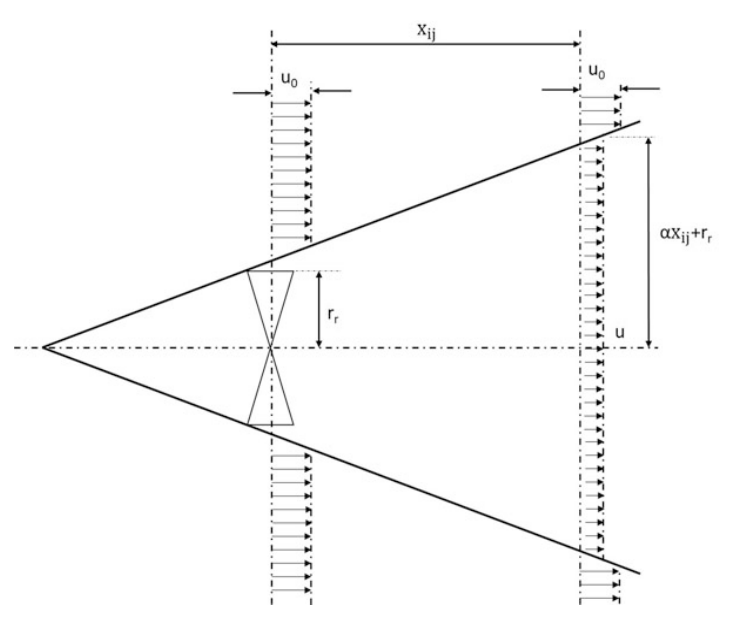
\includegraphics[width=0.9\columnwidth]{Pictures/Wake model.png}
	\figcaption{Wake model~\cite{Karasu2018}}
	\label{fig:pic1}
\end{figure}
\begin{equation}
	\label{eq:2}
	C_T=3.5\cdot\Bigg(\dfrac{2u_{hub}-3.5}{u_{hub}^2}\Bigg)
\end{equation}
\begin{equation}
	\label{eq:3}
	a=0.5\bigg(1-\sqrt{1-C_T}\bigg)
\end{equation}
and $a$ is the wake spreading or entrainment constant, and shows how fast the wake
expands. It can be calculated from Eq.~\eqref{eq:4}.
\begin{equation}
	\label{eq:4}
	\propto=\dfrac{0.5}{\ln}\Bigg(\dfrac{\mathcal{Z}_H}{\mathcal{Z}_0}\Bigg)
\end{equation}
Here, $z_0$~(m) represents the surface roughness height of the site, and $z_H$~(m)
represents the hub height of the wind turbine.
$x_{i,j}$ is the distance between the turbine $i$ and $j$ , and it is calculated based on the
given wind direction $\theta$ (\textit{degree}). Details of Eq.~\eqref{eq:5} can be found in Kusiak and
Song's~\cite{Kusiak2010} paper.
\begin{equation}
	\label{eq:5}
	x_{i,j}=|(x_i-x_j)\cos\theta+(y_i-y_j)\sin\theta|
\end{equation}   
In order to calculate the produced power from a wind turbine, it should be
ensured whether the wind turbine is located in the wake of other wind turbine(s)
or not. To illustrate the wake area behind a wind turbine, an imaginary cone can be
\begin{figure}[h!]
	\centering
	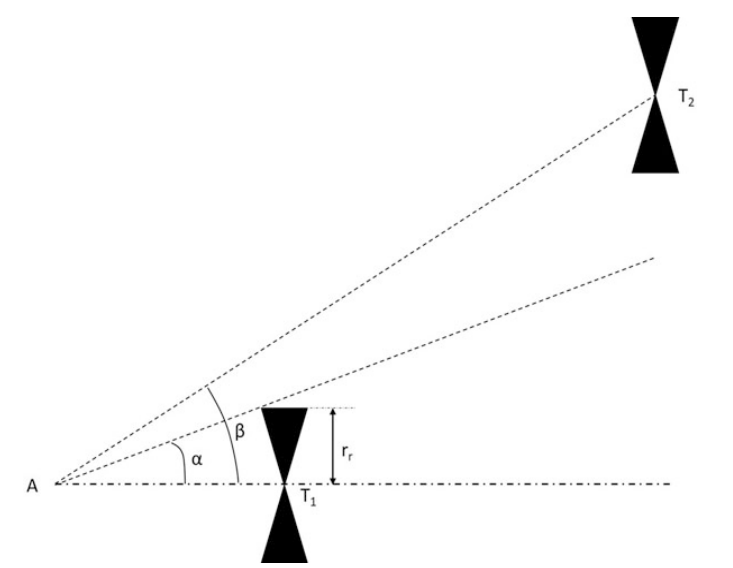
\includegraphics[width=0.9\columnwidth]{Pictures/Imaginary cone of a wind turbine.png}
	\figcaption{Imaginary cone of a wind turbine~\cite{Karasu2018}}
	\label{fig:pic2}
\end{figure}
drawn, see in Fig.~\ref{fig:pic2}~\cite{Karasu2018}. Wind blows from left with a given wind direction $\theta$ . Any
two turbines $i$ and $j$ positioned perpendicular to the wind direction and locate at $(x_i,y_i)$ and $(x_j, y_j)$, respectively. 
The point $A$ is the imaginary vertex, the angle $\alpha\bigg(0\leqslant\alpha\leqslant\dfrac{\pi}{2}\bigg)$
is calculated as $\arctan(\alpha)$, and the distance between $A$ and the hub is $\dfrac{r_r}{\alpha}$.
$\beta(0\leqslant\beta\leqslant\pi)$ is the angle used to determine if turbine $i$ is in the cone of turbine $j$
given the wind direction $\theta$ . For example, in Fig.~\ref{fig:pic2}, if the angle between the vectors
$AT_2$ and $AT_1$ which is $\beta$ is greater than the angle $\alpha$, then $T_2$ will not be inside the
cone, which means $T_2$ will not be under the wake of $T_1$ . On the contrary, if $\beta$ is
smaller than the angle $\alpha$, then $T_2$ will face velocity deficit due to wake effect of $T_1$.
The calculation of the angle $\beta$ is shown in Eq.~\eqref{eq:6}. $a_1=(x_i-x_j)$ $b_1=(y_i-y_j)$
\begin{equation}
	\label{eq:6}
	\beta_{ij}=\cos^{-1}\left(\dfrac{a_1\cos\theta+b_1\sin\theta+\dfrac{r_r}{\propto}}{\sqrt{(a_1+\dfrac{r_r}{\propto}\cos\theta)^2+(b_1+\dfrac{r_r}{\propto}\sin\theta)^2}}\right)
\end{equation}
Large wind farms experience a cumulative effect of multiple wakes. When many
turbines are located in a wind farm, the direction of the wind changes regularly, that
causes certain turbines to be in the wake of other turbines. In this case, multiple
wakes have to be considered. $u_i$~(m$/$s) which is the downstream wind speed of the
turbine $i$ can be calculated by Eq.~\eqref{eq:7}.
\begin{equation}
	\label{eq:7}
	u_i=u_0(1-vel\_def_{ij})
\end{equation}
And the calculation of multiple wake deficits on turbine $i$ can be seen in Eq.~\eqref{eq:8}.
\begin{equation}
	\label{eq:8}
	vel\_def_{i}=\sqrt{\sum\limits^{N}_{j=1,j\neq i,\beta_{ij}<\propto}vel\_def_{ij}^2}
\end{equation}





%%% --------------------------------------------------------
\subsection{Power Model} \label{subsec:powermodel}
%%% --------------------------------------------------------
The power production, $P$~(Watt), from a single wind turbine is given in Eq.~\eqref{eq:9}.
\begin{equation}
	\label{eq:9}
	P=0.5\rho\pi r_r^2u^3C_p
\end{equation}
where $\rho$~(kg$/\text{m}^3$ ) is the air density, and power coefficient $C_p$~(\textit{unitless}) is the fraction
of available power in the wind that captured by the turbine. This stands for turbine
power conversion efficiency which is $42$~\% in this problem.
Total power generated in a wind farm is the sum of individual turbine powers.
As wind flows through a turbine, the volume of air downwind of the turbine has
a lower wind speed and higher turbulence than wind in the freestream. So each of
the turbines may be subjected to different wind speeds caused by wakes, otherwise
power is calculated using the freestream speed, $u$, as Eq.~\eqref{eq:10}.
\begin{equation}
	\label{eq:10}
	P(u)=
	\begin{cases} 
	0\text{~kW},\: u<3.5\\
	0.73u^3\text{~kW},\: 3.5\leqslant u<13 \\
	850\text{~kW},\: 13\leqslant 0<20 \\
	0,\: u\geqslant 20
	\end{cases}
\end{equation}
\begin{equation}
	\label{eq:11}
	P_{tot}=\sum\limits^{N}_{i}P_i
\end{equation}
where $N$ is the total number of wind turbines. And the objective function is
$$\max\sum\limits^{N}_{i}P_i$$





%%% --------------------------------------------------------
\section{Methodology} \label{sec:methodology}
%%% --------------------------------------------------------
%%% --------------------------------------------------------
\subsection{Problem Formulation} \label{subsec:problemformulation}
%%% --------------------------------------------------------
In this paper, a $350\times1000$~m of a wind farm site is considered. Terrain data is
digitized from a map in Google Earth. First, desired terrain is scanned by Path
command, and a set of $1568$~scanned data is collected. This data consists of
latitude, longitude, and elevations. However, latitude and longitude values are both
angles in radians, while corresponding elevations are in meters. Due to the different
dimensions of the data, it is necessary to convert the coordinate data into metric
system. In order to do this, geodesic distances between latitude and longitude points
on the earth's surface should be calculated.
Several approaches can be found in literature for the calculation of distance on
earth surface. Since the earth is not a perfect sphere, and the radius of the earth varies
at the poles and the equator, the Vincenty formula given in Eq.~\eqref{eq:12} and Eq.~\eqref{eq:13} 
is used in this paper. Because this approach models the earth as ellipsoidal, and takes
into account the earth's ellipticity~\cite{Veness2017}. $a_1=\cos\phi_2\times\sin(\varDelta\lambda)^2$, 
$b_1=\cos\phi_2\times\cos(\varDelta\lambda)^2$
\begin{multline}\label{eq:12}
	\varDelta\sigma=\\
	=\arctan\dfrac{\sqrt{a_1+(\cos\phi_1\times\sin\phi_2-\sin\phi_1\times b_1)}}{\sin\phi_1\times\sin\phi_2+\cos\phi_1\times\cos\phi_2\times\cos(\varDelta\lambda)^2}
\end{multline}
$\varDelta\sigma$ is the central angle, $\lambda_1$ and $\lambda_2$ are longitude of the points, $\phi_1$ and $\phi_2$ are latitude
of the points, and all of them are angles in radian. The arc length or the distance,
$d$, is the multiplication of earth mean radius, $r$, by the central angle between two
points, given in Eq.~\eqref{eq:13}.
\begin{equation}
	\label{eq:13}
	d=r\times\varDelta\sigma
\end{equation}
After calculating the distances between the points, the dataset turns into a digital
elevation model (DEM) by Surfer which is a $3$D mapping software program.
The DEM is a representation of the terrain with elevations at regularly spaced
intervals. Wireframe model in Fig.~\ref{fig:pic3} and surface model in Fig.~\ref{fig:pic4} are given to
illustrate the geographical formation of the terrain. Based on this formation the wind
characteristics, disturbed and undisturbed wind flow are modeled. The difference
between the maximum and the minimum altitude within the area is $70$~m. The hourly
average wind speeds and directions for a whole year have been supplied from a $10$~m
met mast from the portal of national meteorological station~\cite{Meteoroloji2016}, and the annual
average wind speed is found $6.2$~m$/$s. In wind direction analysis, the wind rose split
sixteen equal sectors. Winds are frequently oriented in the North (N) with $29.45$~\%,
North North West (NNW) with $29.53$~\%, and North West (NW) with $33.08$~\%, while
the remaining $7.94$~\% is blown from the other $13$ sectors.
The aim of the problem is to find how many turbines can be installed at most
in a given terrain, and give an opinion to the wind farm investor that how many
installation of them would be feasible. In the literature, most of the studies take into
account subdividing the available terrain into cells. The size of a cell is accordingly
chosen to keep the minimum distance between two adjacent turbines, and every
turbine can be installed only at the center of a cell. So the available positions are
finite in a given wind farm site. However, in this study every single point of the
terrain is considered as a possible turbine location. Extraction of the wind farm
contour provides the opportunity to make the search space continuous. Thus, it is
\begin{figure}[h!]
	\centering
	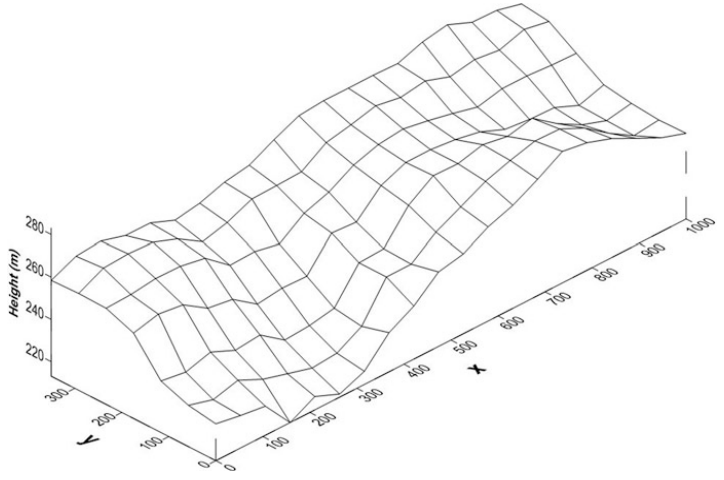
\includegraphics[width=0.9\columnwidth]{Pictures/3D wireframe model of wind farm site.png}
	\figcaption{3D wireframe model of wind farm site}
	\label{fig:pic3}
\end{figure}
\begin{figure}[h!]
	\centering
	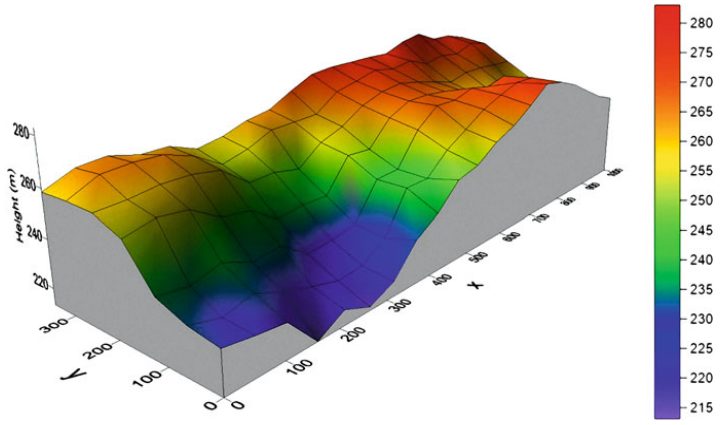
\includegraphics[width=0.9\columnwidth]{Pictures/3D surface model of the wind farm.png}
	\figcaption{3D surface model of the wind farm}
	\label{fig:pic4}
\end{figure}
clear that due to more flexibility in placing wind turbines, more wind turbines can be
placed in a given wind farm. The wind speeds of each point of dataset are calculated
based on power law wind profile. One single type of wind turbine is considered for
the wind farm, and its features are displayed in Table~\ref{tab:1}.
\begin{wraptable}{o}{0.5\columnwidth}
	\tabcaption{Features of turbine used in this study}
	\begin{tblr}{|X|X|}
		\hline
		Rated power & $850\text{~kW}$ \\
		\hline
		Cut-in wind speed & $3.5\text{~m$/$s}$ \\
		\hline
		Rated wind speed & $13\text{~m$/$s}$ \\
		\hline
		Cut-out wind speed & $20\text{~m$/$s}$ \\
		\hline
		Hub height $(\mathcal{Z}_H)$ & $50\text{~m}$ \\
		\hline
		Rotor radius $(r_r)$ & $30\text{~m}$ \\
		\hline
		Power coefficient $(C_P)$ & $0.42$ \\
		\hline
	\end{tblr}
	\label{tab:1}
\end{wraptable}
The minimum turbine installation distance is considered four rotor diameter
($4$D), which is $240$~m. The aim is to create the best layout for the turbines to generate
maximum energy with minimum wake loss. Since wind speed changes with height,
as known as vertical wind shear phenomena, elevation values are utilized. Thereof,
a new approach based on the elevation values of the terrain is proposed to obtain
an initial population to be optimized by genetic algorithm. Finally, in the lights of
above formulas the velocity deficits and power production of the proposed wind
farm are calculated, and compared.





%%% --------------------------------------------------------
%\subsection{Initial Population Based on Elevation Values} \label{subces:initialpopulation}
%%% --------------------------------------------------------
%\subsection{Genetic Algorithm for Optimization} \label{subces:genetialgorithm}
%\subsubsection{Population Formation}
%\subsubsection{Selection}
%\subsubsection{Crossover}
%\subsubsection{Mutation}
%\subsubsection{Genetic Algorithm Parameters}
%\section{Results and Discussion} \label{sec:results}
%%% --------------------------------------------------------





%%% --------------------------------------------------------
\section{Conclusion} \label{sec:conclusion}
%%% --------------------------------------------------------
In this paper, the WFLO problem which is an important issue that needs to be solved
during the design of a wind farm is described. In large wind farms, wake effects
lead to considerable power loss, for this reason it is desirable to minimize them in
order to maximize the power production~\cite{Samorani2011}. Therefore, wake loss consideration
is getting serious among the wind farm investors, since power production is mainly
based on placing the turbines on the right location. In this paper, a wind turbine
placement model which mainly depends on the number of wind turbines, wind speed
and direction, characteristics of terrain and wind turbine features is addressed. First,
wind farm's geographic position data which are latitude, longitude, and elevation
are generated by scanning a digital map in Google Earth. The latitude and longitude
angles of the terrain are transformed into geodesic distances in meters, so that the
dataset turned into a three-dimensional Cartesian coordinates defined by $(x, y, z)$
in metrics. This dataset is introduced to algorithm as possible installation locations
for WTs. By doing this, a continuous search space is generated which gives the
opportunity to locate the wind turbines more liberate. With the help of Surfer
software, DEM is generated to model the terrain. Since wind speed changes with
height, as known as vertical wind shear phenomena, elevation values are utilized
in heuristic approach. The solution starts based on this heuristic approach which
aims to create initial layouts. Then, the genetic algorithm is proposed to optimize
these initial layouts considering to minimize the wake loss, and maximize the power
production while keeping the minimum distance between two turbines. The power
production of the wind farm is calculated using technical information of WTs, the
wake effects, and wind resource taking into account the multiple wind directions
and roughness of the terrain. For the validation of the offered algorithm, the same
problem solved by only GA. The results showed a hybrid approach including a
heuristic mindset offered better layouts in terms of total wake loss and power
production.
In this study, the developed method has shown promising performance in
different scenarios. Although this paper dealt with an optimization of a rectangle
shape wind farm, the offered contour extraction approach provides the opportunity
to exploit irregular shape wind farm micrositing problem. However, addressing
construction and logistical issues regarding WFLO problem will bring more
sophisticated results for the future studies.





\end{document}